%!TEX root = ./dolgozat.tex

Jelen dolgozat tárgyalja annak szükségességét, hogy az alkalmazás integritása állandóan tesztelve legyen (continuous integration), melynek segítségével a szervezet tagjai állandóan visszajelzést kaphatnak az éppen folyamatban lévő fejlesztések, javítások állapotáról. Továbbá a DevOps irány az, amellyel a visszajelzés, a hibajavítás és önmagában a reakcióidő csökkenthető. A keresztfunkciós csapatok meglétével a csapatok horizontális skálázása is lehetővé válik. Az viszont nem került tisztázásra, hogy mindezek hogyan kapcsolódnak össze, hogy válnak valójában elérhetővé és miképpen lehet rájuk minél gyorsabban, transzparensebben reagálni. Ez a fejezet erre hivatott válaszolni, mégpedig a ChatOps irányzattal, amely az angol Chat (beszélgetés) és Ops (operations, üzemeltetés) szavak összevonásából keletkezett.

\section{Kialakulása}

Mind a ChatOps név, mind pedig az első implementáció a GitHub cégnek köszönhető. A cég indulása idején 2006-ban már minden kommunikáció az egyik népszerű chat szolgáltatás segítségével (Campfire) történt. A cég növekedésével párhuzamosan egyre több információra volt szükség egy-egy csapatnak a többi csapattól, illetve az üzleti elemzők, a marketing adatigénye azt okozta, hogy a chaten folyamatosan írtak a fejlesztőknek és az adatbázis hozzáféréssel rendelkező kollégáknak az igényükkel, amelyet a termék fejlődése érdekét szem előtt tartva kielégítették (\cite{what_is_chatops_slideshow}). Ez az adatigénylés gyakran csak arra vonatkozott, hogy működik-e a weboldal éppen Japánban, sikerült-e élesíteni a kereséshez kapcsoló hibákat vagy hány fizető felhasználó használta a weboldalt ez előző napon. Ez azt eredményezte, hogy megpróbálták a fejlesztők automatizálni az adatexportálást, azonban ezt nem ad-hoc szkriptekkel tették meg, hanem egy robottal, ami figyel a chaten történő beszélgetésekre és tud rájuk reagálni. Ennek az iránynak több előnye is volt, ugyanis az első adatigénylés után a lekérdezés automatizálásra került, a robot már végre tudta hajtani a lekérdezést, így a fejlesztő kiadta először a parancsot, amelynek hatására a kívánt eredmény láthatóvá vált azonnal chaten. Mindezt látta az is, akinek az információra szüksége volt, így amikor legközelebb ismét felmerült az adatigénye, már nem kellett mások segítségét igénybe venni, hiszen ő maga is végre tudta hajtani az utasítást. \Aref{fig:pager_sup} ábrán látható, ahogy a Campfire chatrendszerben lekérdezésre kerül az incidensek állapota. A robot válasza azt jelenti, hogy jelenleg nincs incidens, tehát minden rendszer megfelelően működik. \\
A másik fontos irány, ami megalapozta a ChatOps létrejöttét az maga az Ops része a szónak, vagyis az üzemeltetés. A GitHub már kezdetek óta a DevOps filozófiát követi, amelynek köszönhetően egy-egy termékeket több csapat is fejleszt, a csapatok tagjai folyamatosan fluktuálódnak, keverednek.  2014-ben egy átlagos héten a fő terméken 67 ember dolgozott (\cite{github_product_team}), amely azt jelenti, hogy a hét bármely időszakában legalább 67 ember állíthatta élesbe a terméket, ugyanis nem csak teljesen kész fejlesztések kerülhetnek élesítésre, köszönhetően a GitHub által is aktívan alkalmazott funkciókapcsolóknak (feature flag)\nomenclature{funkciókapcsoló (feature flag)}{Az élesítésnek egy olyan formája, amely során a funkció elérhető produkciós környezetben, viszont csak a kiválasztott felhasználók számára. A kapcsoló használata bevált módszer a kísérleti-, félkész-, validálás alatt álló funkciók bevezetésére} köszönhetően (\cite{github_feature_flag}). Ahhoz viszont, hogy bárki bármikor élesíthessen egy kész vagy akár csak prototípus szintjén lévő fejlesztést, teljes transzparencia szükséges, minden résztvevőnek látnia kell, hogy éppen valaki élesít vagy valaki már foglalkozik egy élesítés okozta problémával.\\
\Aref{fig:hubot_deploy} ábrán látható, ahogy az élesítés utasítás kiadásra kerül. A jelen esetben egy speciális verziója a kódnak (smoke-perf) az éles szerverek egy részére (fe1) kerül ki, ez a chatben mindenki számára látható és egyértelmű, hiszen csak angol nyelvű kifejezések kerülnek használatra a robot vezérlésére.

\begin{figure}[ht]
  \centering
    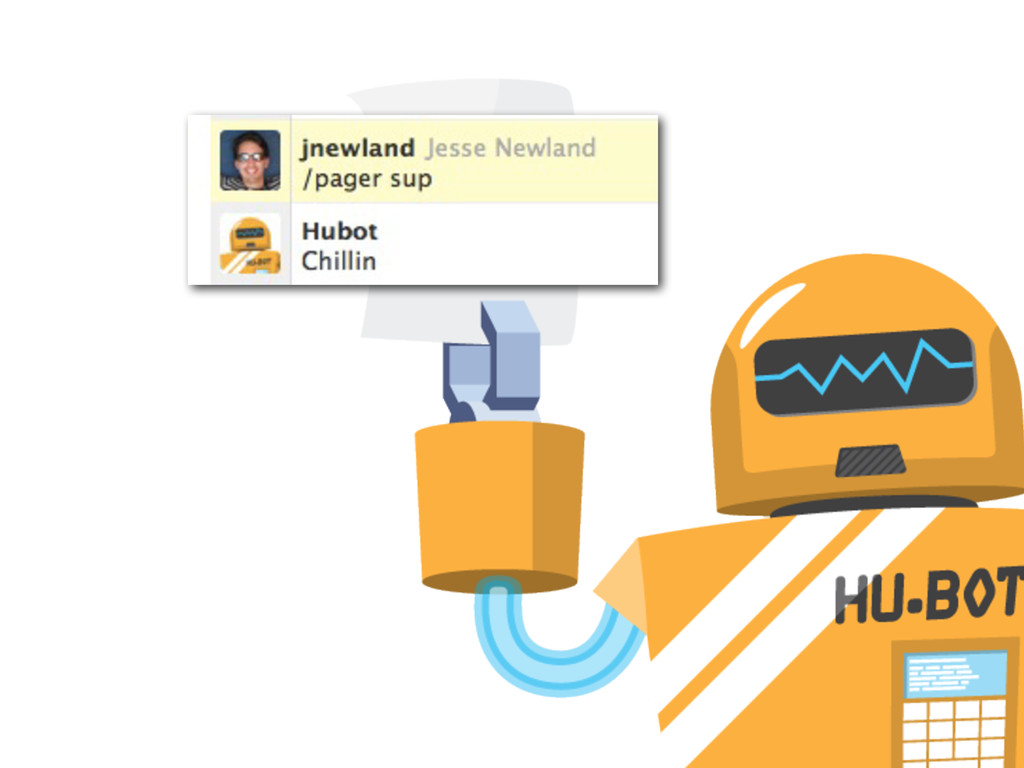
\includegraphics[scale=1.4]{assets/pager_sup.jpg}%
    \caption[DUMMY]%
    {Incidensek lekérdezése Hubot segítségével, forrás: \cite[p.~83]{what_is_chatops_slideshow}}%
    \label{fig:pager_sup}
\end{figure}

\Aref{fig:hubot_status} ábrán viszont már látható, amint egy elrontott élesítés után értesíteni kell az érintetteket, arról hogy a művelet sikertelen volt, ezért vissza kell vonni. Ennek a parancsnak a nagyszerűsége az, hogy nem csak a chaten aktív emberek látják, hanem frissíti a szolgáltatás publikus státusz oldalát is (\url{https://status.github.com}).

\begin{figure}[ht]
  \centering
  \begin{minipage}{.45\textwidth}
    \centering
    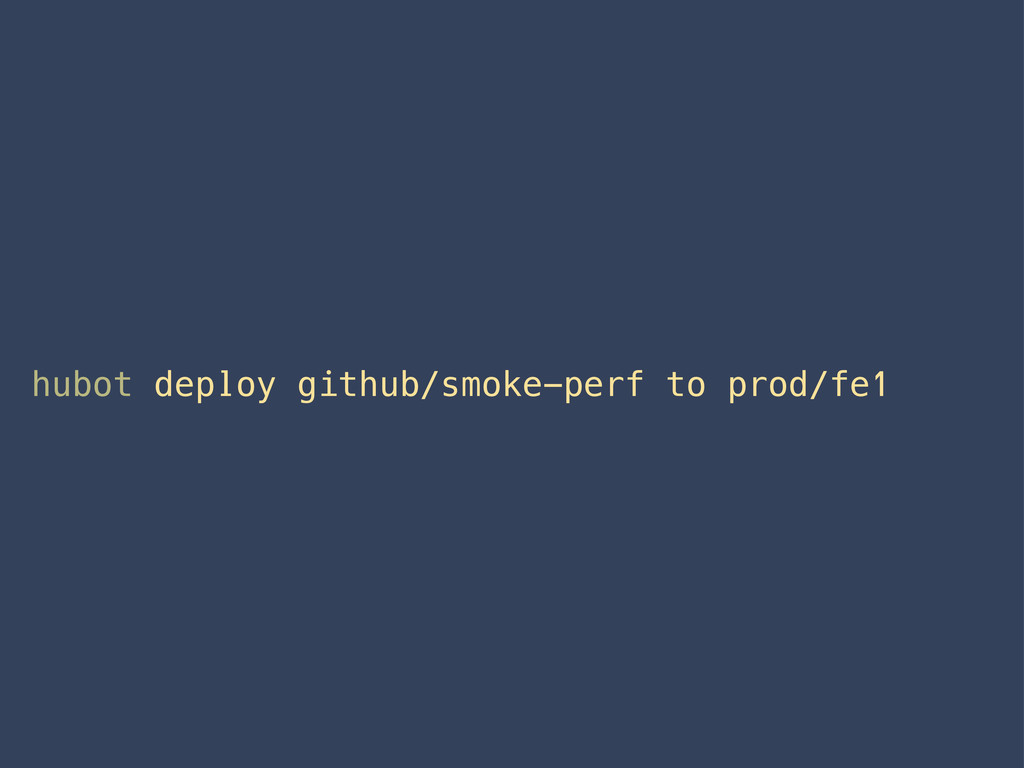
\includegraphics[scale=0.90]{assets/hubot_deploy.jpg}%%
    \caption[DUMMY]%
    {Élesítés robot segítségével,\\forrás: \cite[p.~40]{what_is_chatops_slideshow}}%
    \label{fig:hubot_deploy}
  \end{minipage}\hfill
  \begin{minipage}{.45\textwidth}
    \centering
    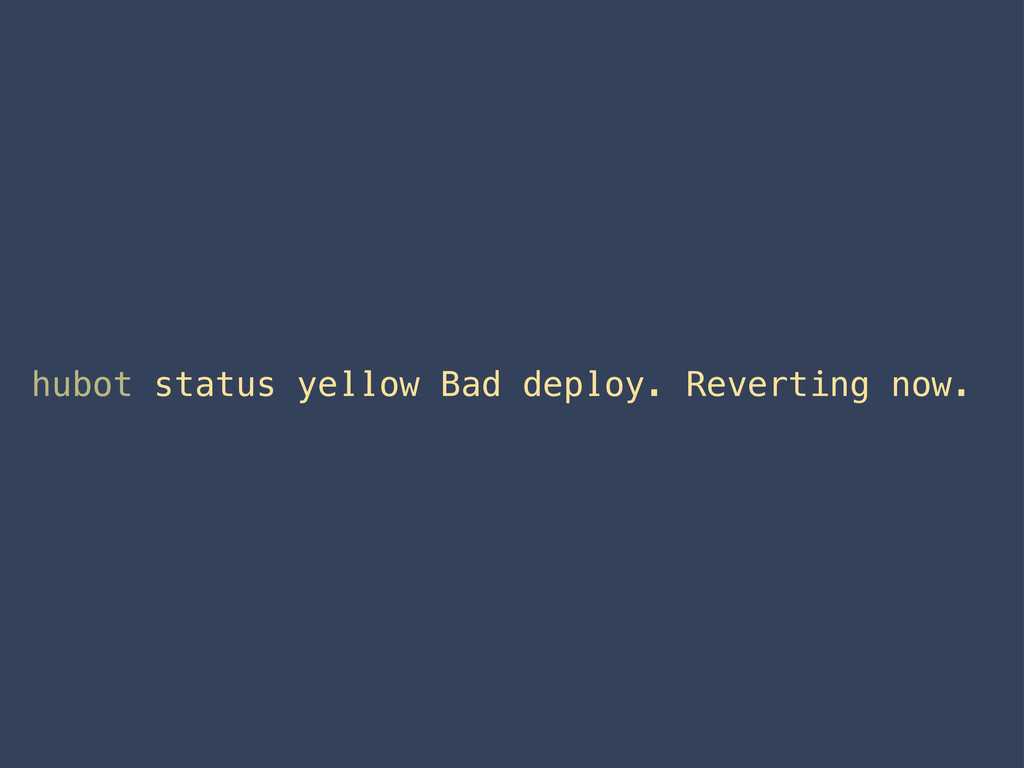
\includegraphics[scale=0.90]{assets/hubot_status.jpg}%
    \caption[DUMMY]%
    {Értesítés rossz élesítésről,\\forrás: \cite[p.~48]{what_is_chatops_slideshow}}%
    \label{fig:hubot_status}
  \end{minipage}\hfill
\end{figure}

\brparagraph{Robot szerepe}
A chatrendszerbe a robot úgy csatlakozik, ahogyan egy ember is tenné, minden üzenet megérkezik hozzá és ezekre reagál. A robot önmagában nem tartalmaz üzleti logikát, mindössze a felhasználók üzenetei alapján képes a programozható interfészekhez (API) hívásokat intézni.

\section{Tulajdonságai}

\brparagraph{Jobb kommunikáció}
\label{subsection:better_communication}
Egy csapatban sok különböző szereplő lehet, amennyiben a csapat agilisan fejleszt, akkor feltehetően lesznek technikai és nem technikai emberek, akik annak ellenére, hogy egy 5-6 fős csapatban dolgoznak differenciált információval és tudással rendelkeznek a terméket illetően. Egy nagyon egyszerű példa, ha a csapat egy olyan termékért felelős, amelyben lehet fizetni, viszont a fizetési szolgáltatás egy hibája, mérhető csökkenést fog okozni a csapat által fejlesztett szoftver mérőszámai alapján. Azonban egy másik szolgáltatás vagy szoftverkomponens állapota könnyen ellenőrizhető egy ChatOps alapú szervezetben, \aref{fig:get_outage_for_payment} példa ezt hivatott bemutatni.

\begin{figure}
    \begin{alltt}
@hubot payment incident? on last week
    \end{alltt}
    \caption[DUMMY]%
    {Az előző heti incidensek listázása a fizetési rendszerhez}%
    \label{fig:get_outage_for_payment}
\end{figure}

Egy másik gyakran előforduló probléma az éjszakai leállások, amikor az ügyeletes akár reggelig a probléma javításán dolgozott és reggel még munkaidő kezdetére nem ért be, akkor könnyen látható, hogy meddig próbálta megjavítani a hibás részt illetve, hogy mit tett a javítás elvégzése érdekében.

\brparagraph{Transzparens}

Az előző pontban kifejtett okok is részben a transzparenciát segítik elő, de a chat rendszer használata már önállóan segíti az átláthatóságot.
Egy szervezet általában sok formáját használja a kommunikációnak:

\begin{itemize}
  \item szöveges üzenetek
  \item tennivalók listája / issue kezelő rendszerek
  \item hibabejelentő rendszerek
  \item telefonhívások
  \item videóhívások
  \item email
  \item sárga cetli
\end{itemize}

Azonban a sok eszköznek köszönhetően biztosan kimaradnak olyan érintettek, akiknek szükségük lenne információra, viszont ha mindezt egy könnyen elérhető felületen keresztül centralizálják, akkor mindenki számára könnyebbé válik az információhoz való hozzáférés.\\
\Aref{lst:search_feature_call} példa kívánja bemutatni, hogy a chat, mint munkaszervezési platform miért tud jól működni. Ha a példában látható Joey és Paul a beszélgetést telefonon vagy emailben ejti meg, akkor Bill semmiképp sem tudott volna csatlakozni a beszélgetéshez, és az implementáció csak egy későbbi szakaszában derült volna fény a Bill által említett problémára.

\begin{figure}
  \begin{alltt}
Joey: @coworker2: We should talk about the new search feature!
Paul: Sure, a quick videocall?
Joey: Sure
Paul: hubot videocall
hubot: Click here to join the video call
       http://videocall.me/conversation/8046741f-1d67
Bill: hey @Joey, @Paul I will join too because I'm going to implement it 
      and there are a few things in the specification which won't work :(
  \end{alltt}
  \caption[DUMMY]%
    {Egy elképzelt beszélgetés, mely jól személteti, hogy a beszélgetéshez, amely elvileg csak Paul és Joey között zajlott volna, még csatlakozott Bill is}%
    \label{lst:search_feature_call}
\end{figure}

Természetesen a centralizálás nem azt jelenti, hogy minden beszélgetést a chaten kell megejteni, hiszen felesleges lenne ennyire központosítani mindent és előbb vagy utóbb feltehetően munkavállalói ellenállás köszönhetően csökkenne a chat használata. Továbbgondolva \aref{lst:search_feature_call} példát, a videóbeszélgetés ugyan nem elérhető chaten, viszont a beszélgetés arról, hogy keresés működésének megbeszélése videóbeszélgetés formájában történt meg az igen, illetve a link a videóbeszélgetéshez (amihez használt szoftver valószínűleg támogatja a videóbeszélgetések rögzítését) elérhető. A példa jól vizualizálja a chat alapú munkavégzés legnagyobb előnyeit: a kronológikus áttekinthetőség, a korábbi beszélgetések kereshetősége, bár ez igaz az emailekre is, viszont itt egy csapat minden tagja megtekintheti, nem csak azok akik rajta voltak a címzett listán.\\

\brparagraph{Egy interfész}
A legtöbb szervezet életében időről időre kerülnek bevezetésre új szoftverek, amelyek betanítási folyamatot igényelnek. Ráadásul ha nehezen illeszkednek a szervezeti kultúrába akkor gyakran a munkavállalók ellenségesen állhatnak a bevezetéssel szemben. Egy nagyon egyszerű példán lehetne ezt szemléltetni, ha be szeretne vezetni a szervezet egy munkaidő nyilvántartó szoftvert, akkor annak feltehetően a kitöltéséhez a következő lépéseket végre kell hajtani:

\begin{description}
  \item[Authentikáció]\hfill\\
  Amennyiben az adott szoftver támogatja, illeszkednie kell a szervezet authenkációjához (LDAP, OpenID), amennyiben ez nem lehetséges abban az esetben a felhasználóknak egy újabb jelszót is meg kell jegyezniük, amely bizonyára nem fogja gyorsítani a bevezetést.
  \item[Érkezés vagy távozás kiválasztása]\hfill\\
  Az érkezés vagy távozás kiválasztása.
  \item[Idő rögzítése]\hfill\\
  Az érkezési vagy távozási idő megadása, esetleg további egyéb megjegyzés kíséretében.
  \item[Kijelentkezés]\hfill\\
  Az alkalmazásból történő kijelentkezés a művelet elvégezése után.
\end{description}
\hfill\\
Ezzel szemben \aref{lst:workhour_with_hubot} ábrán látható egy elképzelt munkaidő nyilvántartás robot segítségével chaten keresztül történő rögzítésel. Könnyen belátható, hogy a robottal történő adminisztrálás sokkal gyorsabb és egyszerűbb, mint egy különálló felületen keresztül.

\begin{figure}
  \begin{alltt}
Bill (08:32): hubot arrived
...
Bill (17:34): hubot leaving for my daughter's violin concert
  \end{alltt}
  \caption[DUMMY]%
    {Munkaidő nyilvántartás chaten keresztül robottal}%
    \label{lst:workhour_with_hubot}
\end{figure}

Természetesen ennek a bevezetése is sokáig eltarthat, hiszen lehet, hogy a szervezet tagjai chaten sem fogják elküldeni az üzenetet a robotnak arról, hogy megérkeztek, mint ahogy a célszoftverbe se lépnének be. Azonban a be nem jelentkezett felhasználókat a szoftver esetleg email utján tudja értesíteni vagy a felettesüket tudja tájokoztatni, addig a robot sokkal jobb felhasználói élmény biztosítása mellett képes ezt megtenni. \Aref{lst:workhour_with_hubot_ux} ábrán ezt lehet megtekinteni. Mivel a chat a kommunikáció központi forrása, ezért a robotnak egyszerűen a felhasználók cselekvéseit kell figyelemmel követnie és azokra reagálnia.

\begin{figure}
  \begin{alltt}
Steve (08:32): <answering question>
Steve (08:35): <asking question>
Steve (08:43): <answering question>
Steve (09:02): <answering question>
hubot (09:02): Hey @Steve it seems you've been here for 30 minutes
               but you haven't checked in yet, shall you?
Steve (09:02): hubot arrived at 08:32
    \end{alltt}
    \caption[DUMMY]%
    {A munkaidő nyilvántartás bevezetése sokkal felhasználóbarátabb tud lenni egy robot segítségével}%
    \label{lst:workhour_with_hubot_ux}
\end{figure}

Ezen túl egyre több szervezetben a szervezet tagjai már nem csak asztali eszközökön kapcsolódnak az internetre, hanem több eszközről. Ilyen például a BYOD (Bring Your Own Device)\nomenclature{BYOD (Bring Your Own Device)}{Olyan vállalati szabályozás, amely megengedni, hogy a szervezet tagjai a saját eszközeiket használják a vállalati adatok és rendszerek elérésére. Mivel a munkavállalók a céges szabályok ellenére is magukkal viszik az eszközeiket, ezért inkább támogatják őket a szervezetek, ahelyett hogy korlátoznák a használatukat.} irányzat, amellyel azokat a céges szabályokat illetik melyek megengedik, hogy a munkavállalók saját személyes eszközeiket használják a munkavégzéshez, azonban ez lehet:

\begin{itemize}
  \item asztali számítógép
  \item notebook
  \item mobiltelefon
  \item okosóra
  \item tablet
  \item könyvolvasó
\end{itemize}

A lista hosszának csak a képzelet, illetve az elérhető internet képes eszközök számossága szab határt. Ezt a számot csak többszörözi az a tény, hogy ezek az eszközök különböző operációs rendszerek különböző verzióit futtatják. Ezek alapján is könnyen belátható, hogy mennyivel egyszerűbb egy szöveges kommunikációra szakosodott chat rendszert használni, mint egy saját felhasználói interfésszel rendelkező rendszert bevezetni, amely feltehetően nem is fogja támogatja az elérhető eszközök töredékét sem.\\
\newline
Természetesen nem minden szoftver helyettesíthető mindössze egy pár szöveges utasítással, azonban érdemes belegondolni, hogy sok kis adminisztrációs rendszer sokkal felhasználóbarátabb és akár erőforrástakarékosabb lenne, ha csupán néhány parancs kiadásával lehetne irányítani ahelyett, hogy egy komplex felületen keresztül lehet őket elérni, amely ráadásul csak az asztali gépen meghatározott böngészőből érhető el.

\brparagraph{Absztrakció}
Az absztrakció építése mindig költséges, de a szervezet jövőbeni lehetőségeit nagyban növeli. Ha a fent említett munkaidőszervezési példánál maradva a szervezet a külső szoftver mellett dönt. Viszont ha egy év után arra a döntésre jut a szervezet, hogy a munkaidőnyilvántartás szükséges, viszont a használt szoftvert lecseréli egy jobb piaci ajánlatnak köszönhetően, akkor számolnia kell a munkavállalókban keltett, újabb szoftver bevezetése okozta frusztrációval.\\
Ha viszont a munkaidőnyilvántartás chaten keresztül kerül megoldásra, a háttérben lévő implementáció vagy szoftver könnyen cserélhető, hiszen dolgozók előtt rejtve volt eddig is, ezért nem is fogják észrevenni, hogy mi történt a háttérben (a használatához szükséges parancsok módosítása nem szükséges).

\brparagraph{Aszinkron kommunikáció}

A kommunikációt két részre lehet tagolni a résztvevő felek időbeosztása alapján: szinkron és aszinkron. A szinkron kommunikáció során a résztvevő feleknek az időbeosztása meg kell, hogy egyezzen, azaz az egyik résztvevő fél kérdésére a másik résztvevő fél azonnal válaszol, tehát a válasz megérkezésének késésétől el lehet tekinteni, azaz nullának tekinthető. A kérdező résztvevő azonnali válaszadásra számít a válaszoló részéről, így működik a szóbeli beszélgetés.\\
Ezzel ellentétben az aszinkron kommunikáció során a résztvevő felek nem számítanak azonnali reakcióra, ilyen kommunikációra példa az email, amely elküldése után a küldő tisztában van vele, hogy a válasz megérkezése és az elküldés között eltelt idő több mint nulla lesz.\\
\newline
Szinkron kommunikáció jellemzői:

\begin{itemize}
  \item a résztvevő felek időben egyszerre vesznek részt a kommunikációban
  \item gyors módja a kommunikációnak
  \item rövid reakcióidő
  \item erős egymásrautaltásg
  \item nagy információáramlás
  \item párhuzamosan csak egy kommunikációban lehet részt venni
  \item jellemző típusai:
  \begin{itemize}
    \item személyes találkozás (több ember esetén megbeszélés)
    \item hívás (videó, hang)
  \end{itemize}
\end{itemize}
A szinkron kommunikáció jellemzően gyors, pörgős, információgazdag, viszont cserébe nagy koncentrációt igényel az idő egy bizonyos pontjától (kommunikáció kezdete) egy másik pontjáig (kommunikáció vége). Egy szervezet esetében ezek a meetingek, szemtől szembe lezajló beszélgetések, brainstorming vagy akár videó- vagy audióhívások lehetnek; egyetemen a tanórák, a csoportos projektfeladatok jó példák a szinkron kommunikációra.\\
\newline
Aszinkron kommunikáció jellemzői:
\begin{itemize}
  \item a résztvevő felek eltérő időben vesznek részt a kommunikációban
  \item lassú módja a kommunikációnak
  \item hosszú reakcióidő
  \item párhuzamosan több kommunikációban is részt lehet venni
  \item elosztott kommunikáció
  \item közvetett egymásrautaltság
  \item alacsonyabb szintű információáramlás
  \item jellemző típusai:
  \begin{itemize}
    \item email
    \item SMS
    \item chat üzenet
    \item levél
  \end{itemize}
\end{itemize}

Az aszinkron kommunikáció jóval lassabb, mint a szinkron, viszont időben nincsenek a résztvevők megkötve, amely természetesen azt jelenti, hogy a reakcióidő megnőhet, illetve lassabb lehet a kommunikáció, csökkenhet a hordozott információmennyiség.\\
\newline
Az előző felsorolás alapján könnyen látható, hogy a szinkron kommunikáció sokkal hatékonyabb és gyorsabb, mint aszinkron társa, azonban sok esetben a szinkron nem megvalósítható, illetve nagyobb erőforrás igénnyel rendelkezik, mint az aszikron. A következő példák ezt kívánják bemutatni:

\begin{description}
  \item [Földrajzilag elosztott csapatok esetén] \hfill\\
  Földrajzilag elosztott csapatok vagy csak ideiglesen eltérő időzónában lévő csapatok esetében a szinkron kommunikáció gyakran nem lehetséges, hiszen 9 órás időeltolódás esetén a munkavégzést megnehezíti, ha egymásra kell várni.
  \item [Más feladat végzése közben] \hfill\\
  A szinkron kommunikáció hatékonyságával vetekedni valóban nem lehet, viszont a szinkron kommunikáció azt jelenti, hogy a kommunikáció megkezdésekor végzett feladatot meg kell szakítani (legalább ideiglenesen), kommunikálni kell, majd a kommunikáció végeztével lehet folytatni a korábban végzett feladatot, amely könnyen belátható, hogy sok megszakításnál a feladat el nem végzésébe torkollhat.
  \item [Információ hiányában] \hfill\\
  Amennyiben a kommunikációt kezdeményező félnek a kérdésére vagy adatigénylésére a válasz hosszabb ideig tart, ez akár lehet pár perc, óra, napok vagy hónapok, akkor az aszinkron kommunikációnak nincs alternatívája. 
\end{description}

Minden feladat nem rendezhető csak szinkron vagy aszinkron csoportba, ezért érdemes a két kommunikációs formát keverni és egy megfelelő mixet kialakítani, amelyet hozzá lehet illeszteni a szervezeti kultúrához. A túlzásba vitt szinkron kommunikáció azt jelenti, hogy a szervezet rengeteget fog kommunikálni, viszont a feladatok nem lesznek elvégezve a sok megszakításnak köszönhetően. Amennyiben az aszinkron irány erősödik meg, akkor a döntések meghozatala fog lelassulni vagy információhiányos állapotban kerülnek a döntések meghozatalra.

Ha a szervezeten belüli szinkron kommunikációt (telefonhívás, videóhívások) sikerül minimalizálni, akkor lehet növelni a szervezet tagjainak terhelhetőségét és minimalizálni az állandóan kontextusváltás okozta frusztrációt, miközben minden kérdés és válasz dokumentálásra kerül a chatrendszernek köszönhetően.

\brparagraph{Tanulva végzett munka - Learning by Doing}
A szervezet felépítésének, mindennapjainak komplexitását jól szemlélteti egy új tag belépése a szervezetbe, akinek meg kell mutatni a munkavégzést. Ezt követketően -az egyedüli használat során- rutin műveletté kell transzformálnia azt, ez mindenki számára nagy stresszor. Hasonlóan problémás lehet, mint a már korábban említett új szoftver bevezetése. Ott bemutatásra is került, hogy miért felhasználóbarátabb egy szöveges üzenetekkel elérhető szoftver.

\begin{figure}[ht]
  \centering
    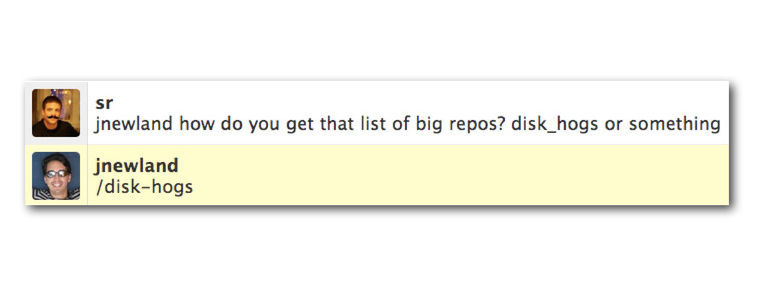
\includegraphics[scale=.6]{assets/github_disk_how_is_it.png}%
    \caption[DUMMY]%
    {Tanulás kommunikáció közben, forrás: \cite[p.~65]{what_is_chatops_slideshow}}%
    \label{fig:learn_by_doing}
\end{figure}

\Aref{fig:learn_by_doing} képen látható beszélgetés a GitHub szervezetében kívánja bemutatni, hogyan tanulnak az emberek miközben végzik a munkájukat. Aki nem ért valamit, kérdezhet és miközben megkapja a választ, már az eredmény is láthatóvá válik. Ha később elfelejtené, akkor bármikor visszalapozhat az első napján született beszélgetések naplójához, amikor megmutatták neki a parancs működését. Továbbá a kereső bárki számára elérhető, és mindenkinek az üzenete elérhető, ezért megnézhető, hogy ki milyen parancsokat használ egy-egy feladat elvégzésére.

\brparagraph{Incidens menedzsment új szintje}
Az incidens menedzsment egy nehéz dolog, ugyanis gyakran éjszaka kell reagálni a felbukkanó hibákra a Runbook\nomenclature{Runbook}{A szoftverek működtetésének és azok működése során fellépő incidensek kezelésének lépéseit tartalmazó gyűjtemény.} által meghatározott módon. A ChatOps előnyeinek felsorolása közül nem véletlen kerül utoljára tárgyalásra ez a fontos terület, ugyanis ebben egyesül a chat alapú munkavégzés a legtöbb pozitív tulajdonsága.\\
Az incidensek megfelelő kezeléséhez szükségesek a következők:
\begin{itemize}
  \item kezelnie kell az incidens hibajegyét
  \item a lehető legtöbb információra van szükség a hibát illetően
  \item az ügyeletet végzőnek tudnia kell értesíteni a felelős csapatot
  \item dokumentálni kell minden elvégzett műveletet
  \item figyelni kell a metrikák (hibaszázalék, válaszidő) változását
  \item küldeni kell értesítést a státusz oldalra
  \item követni kell a Runbook utasításait
  \item ha nem sikerül elhárítani a hibát az ügyelet lejártáig, tájékoztatni kell a következő ügyeletest
\end{itemize}
\hfill\\
\begin{figure}
  \begin{alltt}
hubot (1:12): Failure detected in frontend, alert created with id 1337:
              http://yourduty.com/incident/frontend/1337, @Brian has 
              been alerted
Brian (1:12): hubot pager ack 1337
hubot (1:13): \emph{Incident 1337 has been acknowledged by Brian}
Brian (1:14): hubot graph frontend.http @-1h
hubot (1:14):
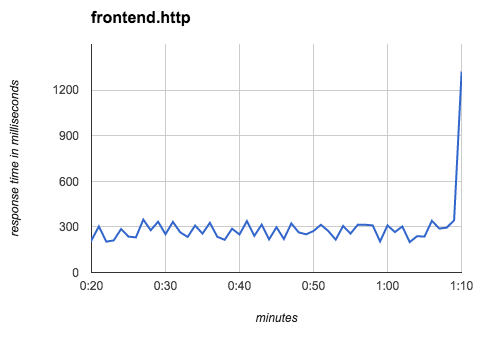
\includegraphics[scale=.6]{assets/frontend_http.png}
Brian (1:15): Something broken for sure, notification should be sent
Brian (1:17): hubot status yellow for frontend 
hubot (1:17): \emph{Status has been set to yellow and team has been notified}
Brian (1:18): Let's see who deployed last time, they rolled 
              out something new
Brian (1:18): hubot deploy frontend
hubot (1:18): Last deploy for frontend was 2 days
Brian (1:18): Nothing happened here, so no new code,
              but something is broken, interesting
Brian (1:24): hubot graph frontend.exception-rate @-1h
....
hubot (3:00): \emph{Oncall rotation has been changed}
hubot (3:00): \emph{Incident 1337 is still active, 
              @Simon has been notified}
Simon (3:00): Popping in, @Brian you can get some sleep
Brian (3:00): Thanks @Simon, I tried my best, the error is still on
  \end{alltt}
  \caption[DUMMY]%
  {Incidens kezelés ChatOps használatával}%
  \label{lst:oncall_message}
\end{figure}

\Aref{lst:oncall_message} beszélgetés jól szemlélteti, hogy a chat segítségével mennyivel könnyebben végre lehet hajtani az elvégzendő a feladatokat.\\
\begin{itemize}
  \item Az értesítés kiküldése után, az incidens kezelése már a robot segítségével elvégezhető.
  \item Az információ összegyűjtése és a metrikák könnyen elérhetőek, mert a grafikonok és a legutóbbi élesítés dátuma lekérdezhetőek egyszerűen chaten keresztül.
  \item A felelős csapat értesítése és a státuszoldal frissítése is a korábban bemutatott módon elvégezhető.
  \item Minden lépés dokumentálva van, ugyanis minden beírt parancs látható mindenki számára (és naplózásra kerül).
  \item A Runbook utasításainak követése is megoldható a robot segítségével, vagy akár a kereső használatával könnyen kideríthető, hogy volt-e már korábban ilyen probléma akár ennél az alkalmazásnál vagy másiknál. Amennyiben volt, az ott használt parancsok használatával is el lehet kezdeni a hibajavítást.
  \item A hiba meg nem javítása esetén nem szükséges felvilágosítani a következő ügyelest, ugyanis az előzmények megtekintésével gyorsan világossá válhat számára is, hogy milyen műveletek lettek végrehajtva a hiba megjelenése óta.
\end{itemize}

Ahhoz, hogy az incidens menedzsment ennyire automatizáltan tudjon működni és ki lehessen használni a chat javára felsorolt előnyöket erős szervezeti támogatottságra van szükség, és a chaten található adatok kell használni, mint az információ egyetlen forrása. Ezen felül minden rendszernek (incidens menedzsment szoftver, monitorozó rendszer, metrika/napló rendszer) rendelkeznie kell programozható interfésszel, melyen keresztül a robot képes az információkhoz való hozzáférést biztosítani.\\
Ebben a részben nem került tárgyalásra, de mindennek a működéséhez szükséges, hogy az alkalmazásokból a megfelelő metrikák beküldésre kerülnek, a hibák a központi naplózó rendszerbe bekerülnek, a monitorozható végpontok nem fals negatív adatokat szolgáltatnak. Ezeknek a megfelelő működése a fejlesztési csapat felelőssége.